\documentclass[../main.tex]{subfiles}
\graphicspath{{\subfix{../images/}}}

\begin{document}
	
\chapter{Methodology}
\section{Introduction}

To evaluate the performance of various support structures developed through topology optimization, a comparative study was conducted in which components fabricated via additive manufacturing were paired with distinct support structures. This investigation assumed that different structural configurations would exhibit varying thermal conductivity, thereby influencing the efficiency of heat dissipation from each material layer during the manufacturing process. Enhanced thermal conduction is anticipated to mitigate overall thermal deformation, as the manufactured component would experience reduced expansion due to a shorter duration of exposure to elevated temperatures.

This section will explain the full process employeds to run the simulations and analyze the resultant data. An overview of the procedural framework is illustrated in Figure~\ref{fig:process_diagram}. The process starts from the creation of the CAD for the manufactured components, followed by the design and CAD creation of the corresponding support structures. The components and the support structures are then merged, and imported into the additive manufacturing software to simulate the results of manufacture. The results obtained from the manufacturing simulation are then subjected to analysis through graphical representations and statistical methods.

\begin{figure}
  \begin{center}
    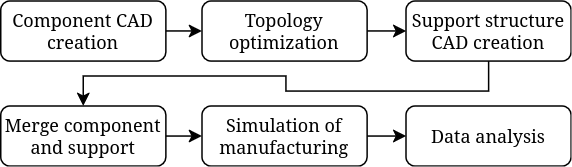
\includegraphics[width=0.90\textwidth]{process_diagram.png}
  \end{center}
  \caption{Process diagram.}\label{fig:process_diagram}
\end{figure}

The subsequent sections explain in detail each stage of this process.

\section{Component CAD}

The components with simple geometries utilized in this study consist of a cube, three triangular
components with different slopes, and three cylindrical components with different values of
curvature. These shapes with these dimenions were chosen to ease the comparison of results between this study and the study of Peishu \cite{chungpei-hsuStudyLatticeSupport2024}. All the CAD models
used for the simple geometry study were created using FreeCAD, an open-source CAD software. The components were exported as .STP files, and then were merged with their corresponding support structures using the software nTop. The geometries used for this preliminary study are the following:

\begin{itemize}
  \item A cube with side length of 30 mm, as shown in Figure \ref{fig:cube}.
  \item Three triangular components with varying slopes. All triangular components have a base of 30 x 30 mm$^2$, with slopes of 15\degree, 30\degree and 45 \degree. The measurements are shown in Figures \ref{fig:tri15}, \ref{fig:tri30},  and \ref{fig:tri45}.
  \item Three prisms with fillets of different. The radii used were 20 mm, 30 mm, and 40 mm. These rounded prisms also have a base of 30 x 30 cm$^2$. They are shown in Figures \ref{fig:cyl20}, \ref{fig:cyl30}, and \ref{fig:cyl40}.
\end{itemize}

\begin{figure}
	\begin{center}
		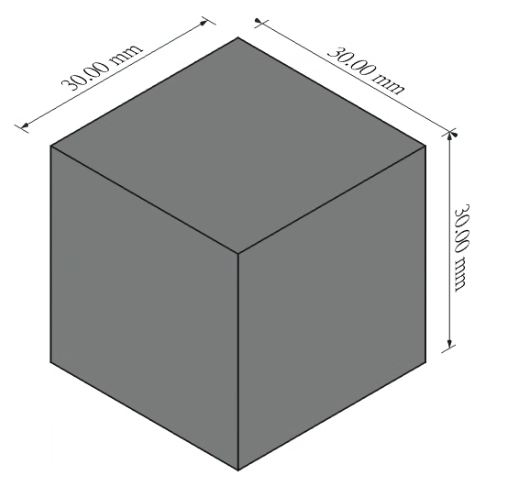
\includegraphics[width=0.40\textwidth]{cube.png}
	\end{center}
	\caption{Dimensions of cube component.}\label{fig:cube}
\end{figure}

\begin{figure}
  \begin{subfigure}{0.3\textwidth}
    \begin{center}
		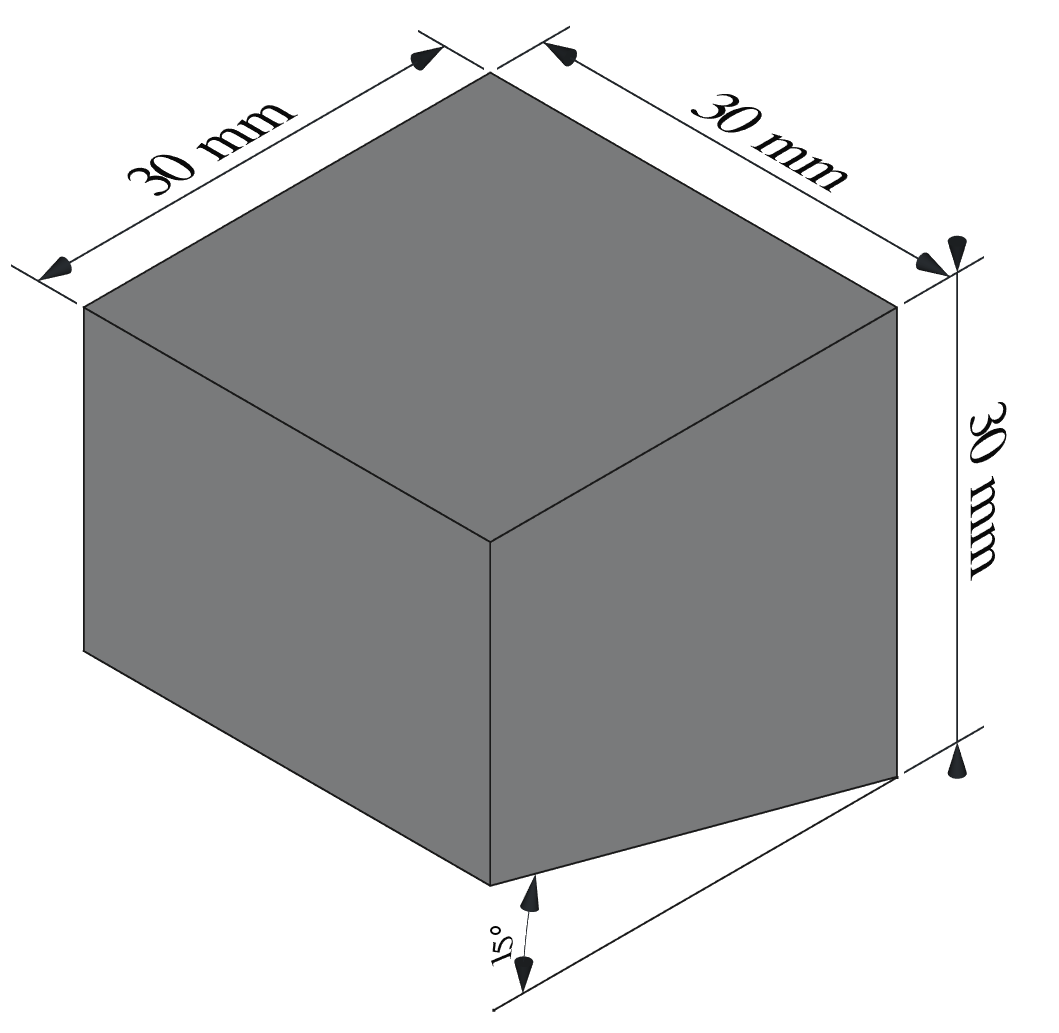
\includegraphics[width=\linewidth]{triangle15.png}
  \end{center}
    \caption{15\degree triangle.}\label{fig:tri15}
  \end{subfigure}
  \begin{subfigure}{0.3\textwidth}
      \begin{center}
      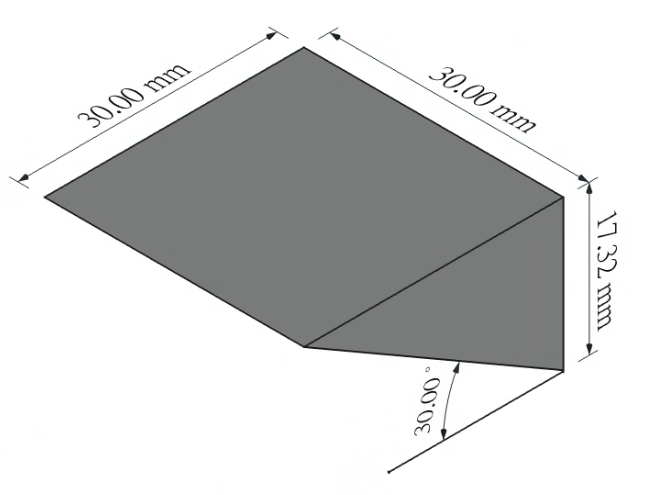
\includegraphics[width=\linewidth]{triangle30.png}
      \end{center}
      \caption{30\degree triangle.}\label{fig:tri30}
  \end{subfigure}
  \begin{subfigure}{0.3\textwidth}
      \begin{center}
      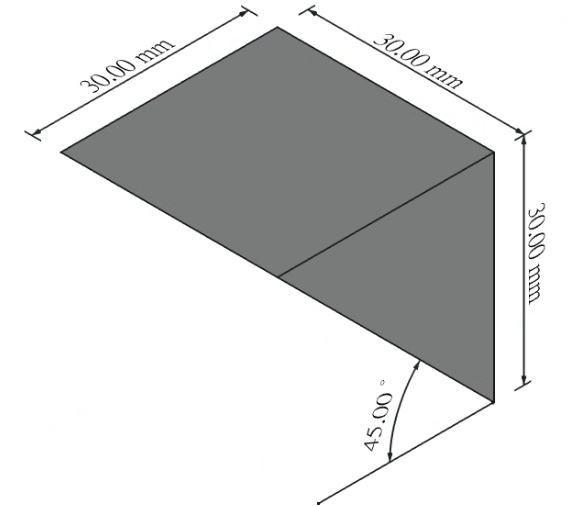
\includegraphics[width=\linewidth]{triangle45.png}
      \end{center}
      \caption{45\degree triangle.}\label{fig:tri45}
  \end{subfigure}
  \caption{Dimensions of triangular parts.}
\end{figure}

\begin{figure}
  \begin{subfigure}{0.3\textwidth}
	\begin{center}
		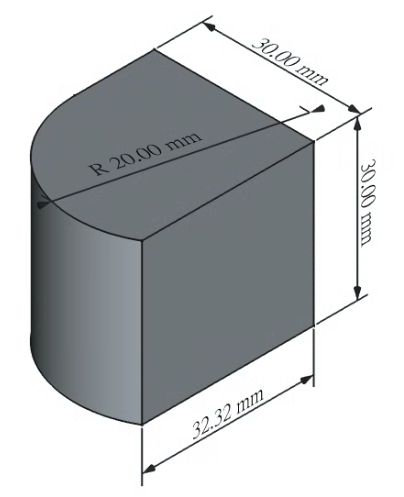
\includegraphics[width=0.9\linewidth]{cyl20.png}
	\end{center}
	\caption{Part with R20 mm fillet.}\label{fig:cyl20}
  \end{subfigure}
\begin{subfigure}{0.3\textwidth}
	\begin{center}
		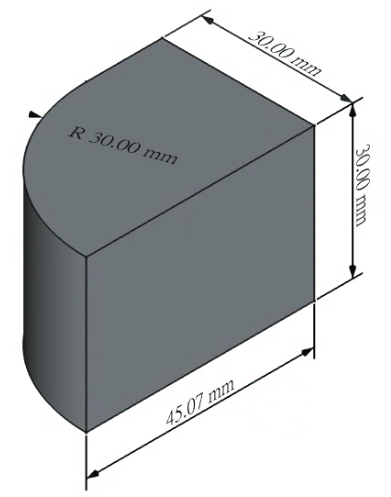
\includegraphics[width=0.9\linewidth]{cyl30.png}
	\end{center}
	\caption{Part with R30 mm fillet.}\label{fig:cyl30}
\end{subfigure}
\begin{subfigure}{0.3\textwidth}
	\begin{center}
		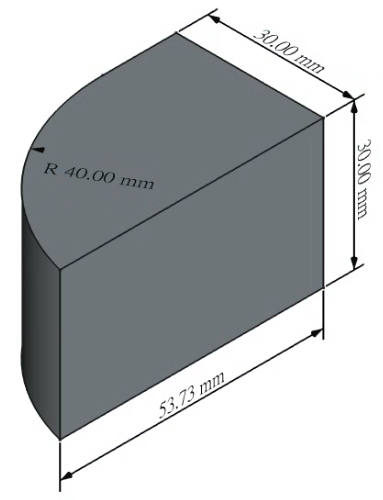
\includegraphics[width=0.9\linewidth]{cyl40.png}
	\end{center}
	\caption{Part with R40 mm fillet.}\label{fig:cyl40}
\end{subfigure}
\caption{Dimensions of rounded parts.}
\end{figure}

Apart from the parts above, a CAD model for a femoral component was also employed. The femoral component is one of the prostethic components used in total knee arthroplasty, and is the piece that is directly connected to the patient's femur. This is shown in Figures \ref{fig:fem1} and \ref{fig:fem2}.

\begin{figure}
  \begin{center}
  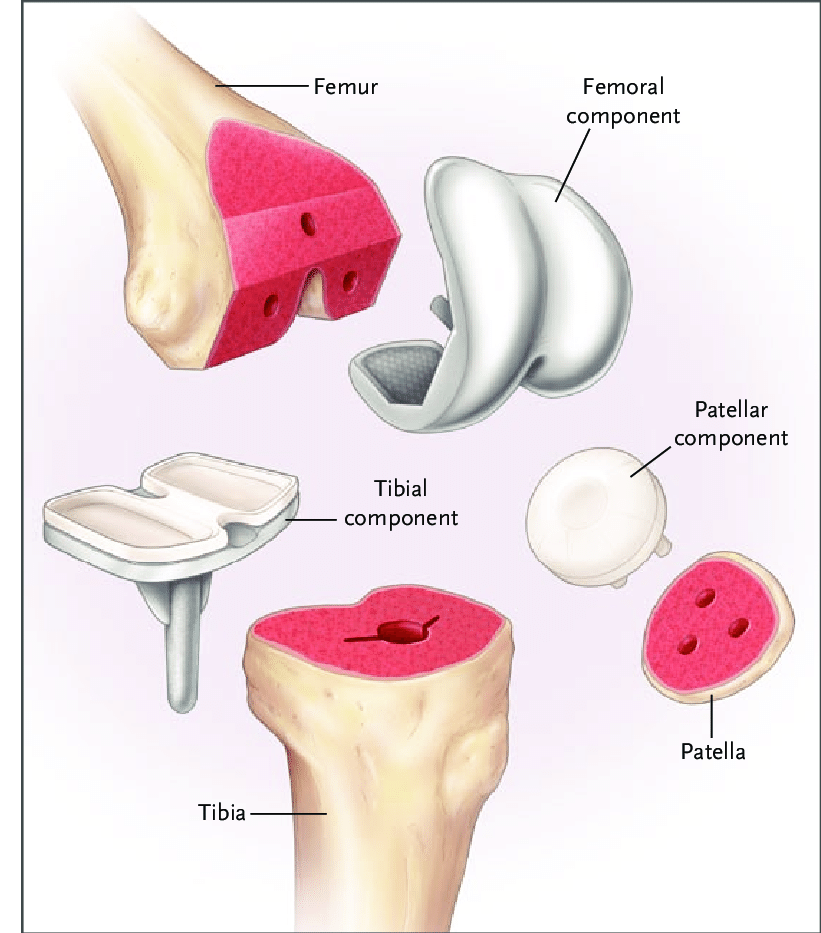
\includegraphics[width=0.45\textwidth]{femoral.png}
\end{center}
  \caption{Components of total knee arthroplasty prothesis. Taken from \cite{leopoldMinimallyInvasiveTotal2009}.}
  \label{fig:fem1}
\end{figure}

\begin{figure}
  \begin{center}
  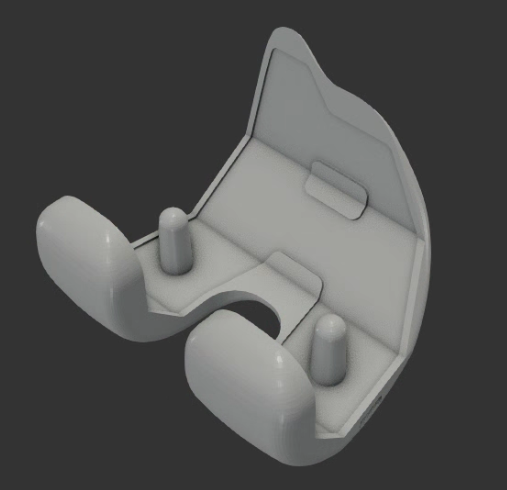
\includegraphics[width=0.45\textwidth]{femoral2.png}
\end{center}
  \caption{CAD model of femoral component.}
  \label{fig:fem2}
\end{figure}

\section{Topology optimization model}

The supporting structures of the components were created using the method of topology optimization. The design was implemented using the topology optimization module of COMSOL Multiphysics 6.2.  

The steps for creating a valid topology optimization model are: determine the design volume, design the support structure using topology optimization, merge the support structure with the part, and carry out the FEM simulation for manufacture.

\subsection{Design domain}

The design domain consisted of the volume between the bottom face of each component and the xy plane, when the component is placed at a height of 30mm above the xy plane. For the simple geometry parts, as they have high symmetry, the design domain was just taken to be a 2D slice of the volume. The topology optimization problem was then solved for this volume, and the resulting topologies were extruded in the direction perpendicular to the design plane to cover the space underneath the part. For the femoral component, the topology optimization was directly solved in the 3D volume between the lower surface of the femoral component and the xy plane. Figures \ref{fig:des1} and \ref{fig:des2} show examples of design domains.


\begin{figure}[h!]
  \begin{subfigure}{0.45\textwidth}
    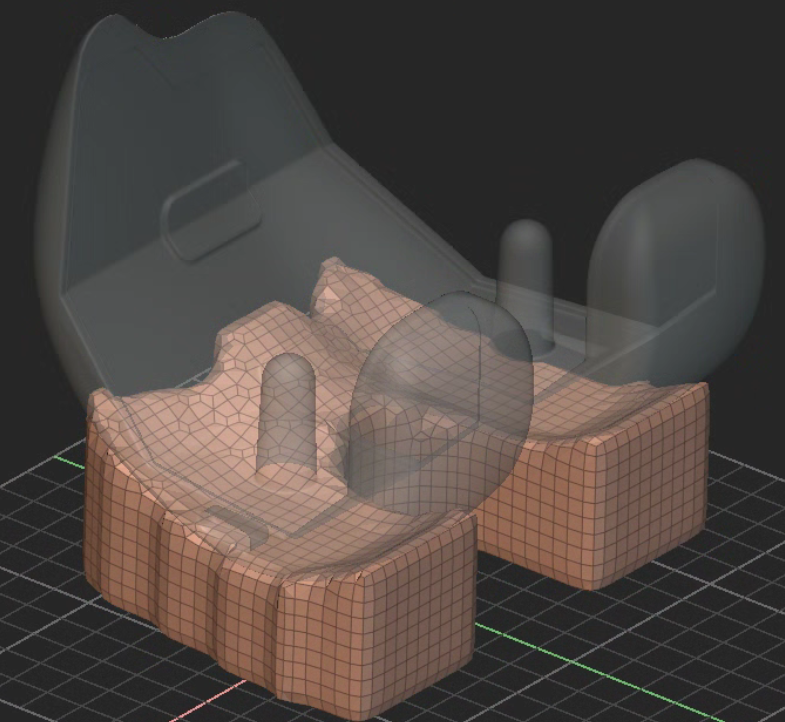
\includegraphics[width=\linewidth]{designdomain3d.png}
    \caption{Design domain for femoral component.}
    \label{fig:des1}
  \end{subfigure}
  \begin{subfigure}{0.45\textwidth}
    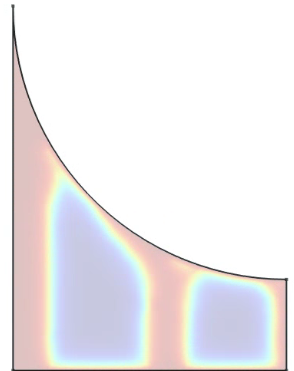
\includegraphics[width=\linewidth]{designdomain2d.png}
    \caption{Design domain for rounded part.}
    \label{fig:des2}
  \end{subfigure}
  \caption{Examples of design domains.}
\end{figure}

\subsection{Objective functions}

The objective of the problem is to maximize the thermal conduction of the support structure, while at the same time maximizing its stiffness. The thermal conductivity has been chosen as an objective since it is required to drive heat away from the part as fast as possible to reduce its thermal deformation. 
Thermal conduction is given by Fourier's law as:

\begin{equation}
  \label{eq:Fourier Law}
  \bm{Q} = -\kappa \nabla T
\end{equation}

where $\bm{Q}$ is the heat conduction through the material, $\kappa$ is the material's thermal conductivity and $\nabla T$ is the thermal gradient. For use in a finite element solver, the objective function $c_t$ and Fourier's law can be written using matrix notation as:

\begin{align}
  \text{minimize} \hspace{0.5cm} & c_t = \bm{T^T} \bm{Q} \\
           & \bm{\kappa}\bm{T}  = \bm{Q},
\end{align}

where $\bm{\kappa}$ is the global thermal conductivity matrix, $\bm{T}$ is the temperature vector, and $\bm{Q}$ is the thermal load, or heat flux, vector. Thermal compliance $c_t$ can be thought of the thermal analogy to the stiffness of a structure. In structural problems, the objective is to maximize the stiffness, or mimize the compliance, as compliance is the inverse of stifness. Similarly, in thermal problems, the objective is to maximize the thermal conductivity, or alternatively, minimize the thermal compliance, which can be though of as the inverse of conductivity. Thermal compliance has extensively been used in other topology optimization problems such as \cite{leeObjectiveFunctionTopology2021}, \cite{yoonTopologicalDesignHeat2010}, and \cite{brunsTopologyOptimizationConvectiondominated2007}.

At the same time, stiffness of the support structure should be be maximized to avoid considerable deformations that might affect the part geometry. The geometry resulting from the thermal optimization could result in thin, dendrite-like structures, which could buckle and collapse under the component's weight, causing the whole manufacturing process to fail. Assuming small deformations, we can express the displacement of the material by using Hook's law,

\begin{equation}
  \bm{F} = k\bm{U},
\end{equation}

where $\bm{F}$ is the force applied, $k$ is the stiffness of a small element, and $\bm{U}$ is the displacement of the element from its equilibrium position. For finite element analysis, the minimization of the compliance $c$ of the structure and its mechanical behavior can be expressed as:

\begin{align}
  \text{minimize} \hspace{0.5cm} & c = \bm{U^T} \bm{F} \\
            & \bm{K} \bm{U} = \bm{F}
\end{align}

where $\bm{K}$ is the global stiffness matrix, $\bm{U}$ is the vector of nodal displacement, and $\bm{F}$ is the vector of loads.

We can therefore combine these two together to obtain the objective function for the topology optimization problem, with $\omega_1$ and $\omega_2$ the weight coefficients that encapsulate the relative importance of each objective:

\begin{equation}
  \text{minimize} \hspace{0.5cm} \omega_1 \bm{T^T} \bm{Q} + \omega_2 \bm{U^T} \bm{F}.
\end{equation}

\subsection{Topology optimization equations}

Having decided the governing equations and objective function for the system, the topology optimzation model must be chosen. For this study, the SIMP approach with a hyperbolic tangent projection has been employed, utilizing a volume fraction restriction. Mathematically, the topology optimization problem can be formulated as follows:

\begin{align}
  \text{minimize}  & \hspace{0.5cm} X_{obj} = \omega_1 \bm{T}^T \bm{Q} + w_2 \bm{U}^T \bm{F}  \\ 
  \text{subject to} & \hspace{0.5cm} \bm{\kappa}(\bm{\tilde{\rho}}) \bm{T} = \bm{Q} \\
                    &  \hspace{0.5cm} \bm{K}(\bm{\tilde{\rho}}){\bm{U}} = \bm{F} \\
    & \hspace{0.5cm} V = \sum _{i \in \mathbb{N}_e } \tilde{\rho_i} v_i \leq V_c  \\ 
    & \hspace{0.5cm} 0 \leq \rho_{min} \leq \tilde{\rho_i} \leq 1, \hspace{0.5cm} \forall i \in \mathbb{N}_e  \\
    & \hspace{0.5cm} \omega_1 + \omega_2 = 1,  
 \end{align}

 where the density $\tilde{\rho}$ has been defined using the hyperbolic tangent projection function as defined in section \ref{ch:threshold}.

\section{COMSOL implementation}

\subsection{Mesh}

To run the topology optimization algorithm and obtain a solution, the design domain must be divided into finite element methods for computation. For the 2D design domains of the simple geometry elements, free triangular meshes were utilized, using a predefined mesh element size of "finer". This resulted in about 2000-3000 elements for each of the design domains, depending on the geometry of the domain. These mesh parameters were chosen to produce fast results and to obtain a general idea of how the simulation parameteres affected the solution of the topology optimization problem. An example of 2D mesh can be seen in Figure \ref{fig:mesh2d}.

\begin{figure}[h!]
  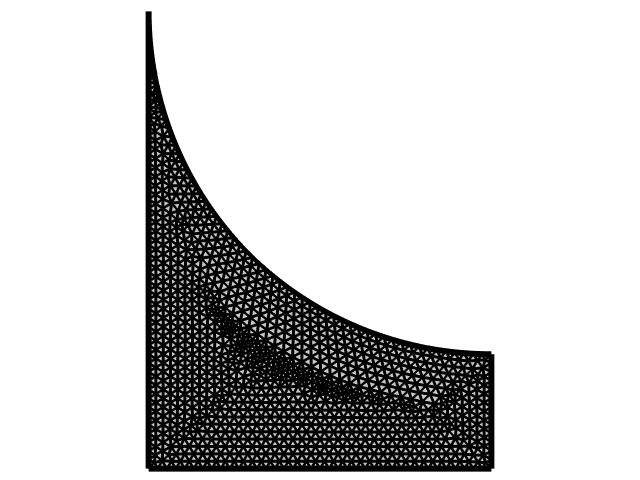
\includegraphics[width=\textwidth]{mesh1.png}
  \caption{Mesh of the design domain for one of the rounded parts.}
  \label{fig:mesh2d}
\end{figure}

On the other hand, For the 3D design domain of the femoral component support structure, the mesh sizing parameters were chosen with more deliberation. The maximum and minimum element sizes of the mesh were determined based on the minimum element size achievable by the selective laser melting (SLM) machine utilized in this study, which is approximately 0.2 millimeters. However, employing a mesh with an element size of 0.2 millimeters results in excessively fine meshes that significantly prolong computational solving times. Consequently, the maximum and minimum mesh sizes were adjusted to be 8 and 4 times the minimum feature size, resulting in values of approximately 1.6 millimeters and 0.8 millimeters, respectively. This resulted in meshes with approximately 164,000 elements. The resulting mesh can be seen in Figure \ref{fig:mesh3d}.

\begin{figure}[h!]
  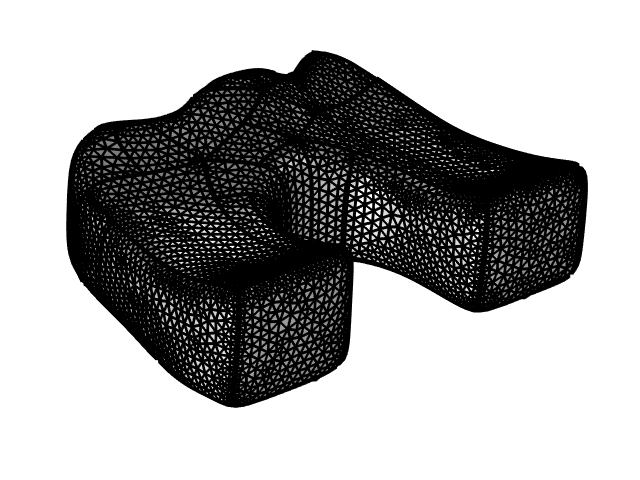
\includegraphics[width=\textwidth]{femmesh.png}
  \caption{Mesh of the design domain for the support structure of the femoral component.}
  \label{fig:mesh3d}
\end{figure}

\subsection{Physical parameters}

For the topology optimization solution to be useful, realistic thermal and stress load should be used. The thermal load was based on the maximum wattage and efficiency of the laser achievable by the selective laser melting machine used in this work. The laser's power is 200 W, with an efficiency of 25\%. This value cannot be used for the thermal load, since the laser is only activated for a small amount of time. From the FEM software building process parameters, each layer is heated for approximately 154 ms. Therefore, with an effective power of 200 W x 0.25\% = 50W, the total amount of energy added to the layer during the heating time is 50 W x 154 ms = 7.7 J. But each layer heating time occurs periodically, with a period of approximately 440 s. Therefore, the average power input to the system per cycle is calculated to be 0.0175 W. The approximate area of the top surface of the support structure design domain is approximately 30 mm x 30 mm = 900 mm$^2$. Diving the power per cycle by this area yields a heat flux of about 19.4 W/mm$^2$, which was rounded up to 20.0 W/m$^2$. For the heat flux used in the femoral component calculation, the difference is in the area of the top surface of the design domain. This area is about 1690 mm$^2$, and thus the heat flux used for the support structure design in accounts to be about 10.37 W/m$^2$, which was rounded to 10 W/m$^2$. A graphical representation of this calculation is shown in Figure \ref{fig:heating}.

The material used in all simulations was 316L stainless steel. This material is often used for medical implants due to its superior mechanical, fatigue, wear and corrosion properties \cite{davisComprehensiveReviewMetallic2022}. The mechanical and thermal properties of 316L steel relevant to this study are shown in Table \ref{tab:316l}.

\begin{table}[h!]
  \centering
  \begin{tabular} { |c | c| }
    \hline
    \textbf{Density} & 8.0 g / cm$^3$ \\
    \hline
    \textbf{Thermal conductivity} & 15 W / (m$\cdot$K) \\
    \hline
    \textbf{Heat capacity} & 500 J / (kg$\cdot$K) \\
    \hline
    \textbf{Young's Modulus} & 200 GPa \\
    \hline
  \end{tabular}
  \caption{Phyiscal properites of 316L steel.}
  \label{tab:316l}
\end{table}

It should be noted that the physical properties of stainless steel shown above are average properties at 20\degree C. These are subject to change during the building process, as the material is repeatedly heated above its melting point and cooled down, but for the purpose of simplifying the simulation process, these constant values were employed for the topology optimization problem. 

\begin{figure}
  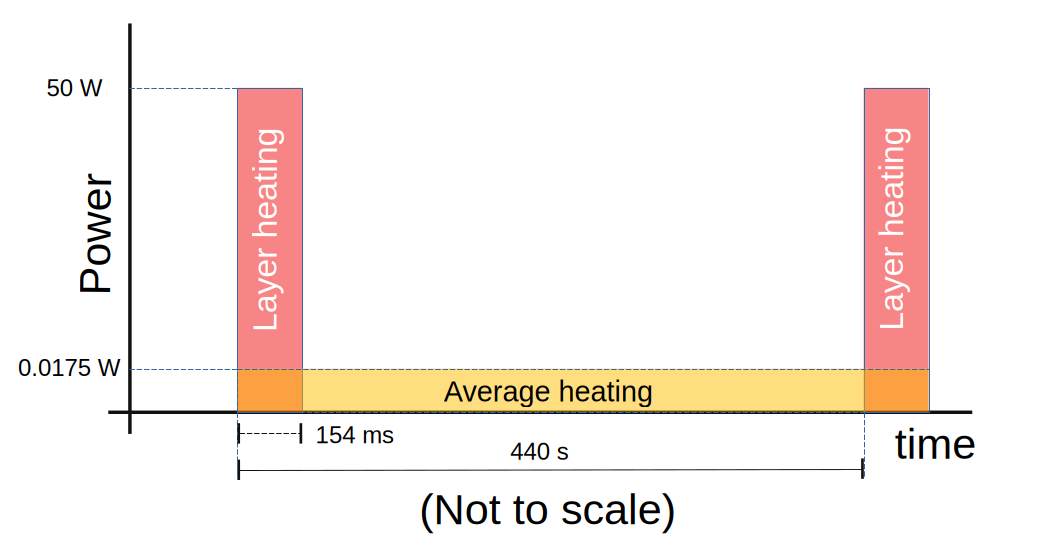
\includegraphics[width=\textwidth]{heating.png}
  \caption{Layer heating cycle.}
  \label{fig:heating}
\end{figure}

For the calculation of compliance, the structural load was also calculated by using the weight of each component and dividing it by the top area of the design domain. All of the components were modeled using the density of 316L steel, which is approximately 7.93 g/cm$^3$. This was then multiplied by the volume of each component to obtain the mass. For example, the. The volume of the femoral component was calculated to be about 32800 mm$^3$, and therefore the mass of the femoral component amounted to 0.263 kg. This was then divided by the top area of the design domain. Taking again the example of the femoral component's support structure, the area of the top surface is about 1690 mm$^2$, and so the average stress value of the top surface is calculated as (0.263 kg)$g$ /1690 mm$^2$ = 1560 N/m$^2$, where $g$ is the gravitational constant. 

\subsection{Parametric study}

The topology optimization problem was solved using COMSOL Multiphysics 6.2 software. COMSOL allows the creation of parametric studies that allow to run a simulation with a list of parameters to be varied, in order to study the influence of different values on the solution of a system. For this study, the values of volume fraction, objective function weights, and hyperbolic tangent angle were chosen as the parameters to be varied.

Volume fraction is defined as the maximum amount of volume that the topology can cover within the design domain. This criteria is chosen because we seek to use less material for the supporting structure, as long as we can maintain the total deformation of the manufacturing componont beneath a threshold. For the simple geometries 50\% and 75\% of volume fraction were considered. For the femoral component study, volume fractions of 25\%, 33\%, 40\%, 50\% and 75\% were considered. 

Finally, the hyperbolic tangent angle projection was also varied. The hyperbolic tangent was varied from a value of 0.001\degree to 8\degree, in steps in 2\degree. The variation was stopped at 8\degree since it was noticed that for $\theta \geq$ 8\degree there would be no discernible differences between results.

Finally, the objective functions weights were also varied for the design of topologies for the simple geometry parts. The pairings of weight used were (0.2, 0.8), (0.5 , 0.5), and (0.2, 0.8), where the first weight in each pair corresponds to the weight of the thermal compliance objective and the second corresponds to the weight of the mechanical compliance objective. All of these parameters are summarized in Table \ref{tab:params}.

\begin{table}
  \centering
  \begin{tabular} { |c| c| c|}
    \hline
    \textbf{Parameter} & \multicolumn{2}{|c|}{\textbf{Values}} \\
  \hline
  \multirow{2}{10em}
    {\textbf{Volume fraction}} & Simple geometry & 0.50, 0.75 \\
                    & Femoral component & 0.25, 0.33, 0.40, 0.50, 0.75 \\
  \hline
    \multirow{2}{10em}{\textbf{Hyperbolic tangent angle}} & Simple geometry & 0.001\degree, 2\degree, 4\degree, 8\degree \\
                                               & Femoral component & 0.001\degree, 2\degree, 4\degree, 8\degree \\
  \hline
    \multirow{2}{10em}{\textbf{Objective weights}} & Simple geometry & (0.2, 0.8), (0.5, 0.5), (0.8, 0.2) \\
                                        & Femoral component & (1.0, 0.0)\\
  \hline
\end{tabular}
\caption{Variation of parameters.}
\label{tab:params}
\end{table}

\subsection{Boundary conditions}

It is possible to change the material boundary conditions in COMSOL when solving the topology optimization problem. As an extra study parameter, the material boundary condition of several edges of the design domain were also varied for this study. For the 2D design domains, different topologies were obtained by having either a prescribed material or void boundary in the side elements of the design domain. For the femoral component, there was no variation in the density of the design domain boundary. Figures \ref{fig:solid} and \ref{fig:void} showcase the difference in topologies by varying the prescribed density on the support structure of the cube part.

\begin{figure}
  \begin{subfigure}{0.45\textwidth}
    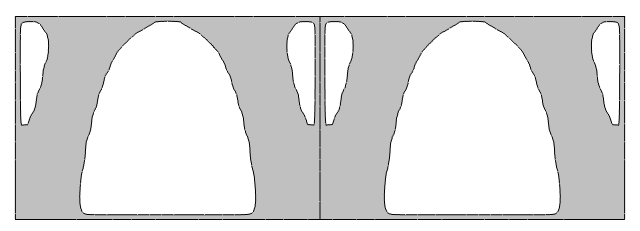
\includegraphics[width=\linewidth]{side_mat_volfrac20.png}
    \caption{Topology with solid material density.}
    \label{fig:solid}
  \end{subfigure}
  \begin{subfigure}{0.45\textwidth}
    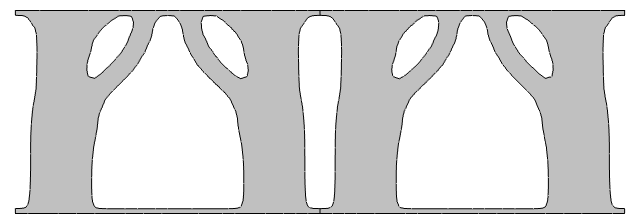
\includegraphics[width=\linewidth]{side_void_volfrac20.png}
    \caption{Topology with void material density.}
    \label{fig:void}
  \end{subfigure}
  \caption{Variation in topology due to material prescribed density at the side boundary of design domain.}
\end{figure}

The heat transfer and solid mechanics boundary conditions must also be specified. The heat transfer problem boundary conditions consisted of a heat flux through the upper surface of 20 W / (m$^2$$\cdot$K) and 10 W / (m$^2$$\cdot$K) for the simple geometry parts and femoral component respectively. The inferior surface was set at a constant temperature of 200\degree K, and the sides were kept insulated.

\begin{figure}[h!]
  \centering
  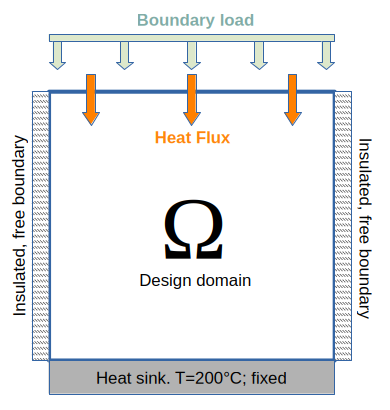
\includegraphics{boundaryconds.png}
  \caption{Boundary condition examples for design domain of cube component.}
\end{figure}

The solid mechanics boundary conditions consisted of a load corresponding to the part's weight on the top surface. The bottom surface was constrained to be a fixed surface with no displacement, and the sides were set to be free surfaces.

\subsection{COMSOL implementation final details}

Once all the physical and material parameters, the topology optimization model and parameters, boundary conditions, and parametric study have been set up, the solver will have all the information needed to obtain a solution. For this project, the solver algorithm utilized the method of moving asymptotes (MMA) \cite{svanbergMethodMovingAsymptotes1987}, with a maximum iteration number of 50. The optimality tolerance was also set to COMSOL's default value of 0.001. Lastly, the penalty factor for the SIMP method was set to p=3.

\begin{figure}
  \begin{subfigure}{0.45\textwidth}
    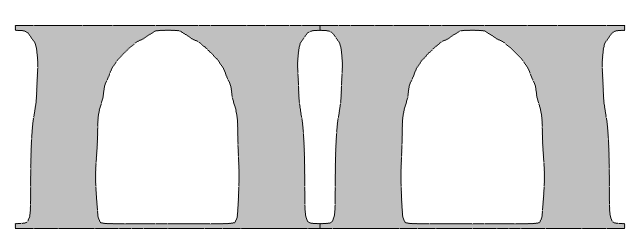
\includegraphics[width=\linewidth]{excube.png}
  \end{subfigure}
  \begin{subfigure}{0.45\textwidth}
      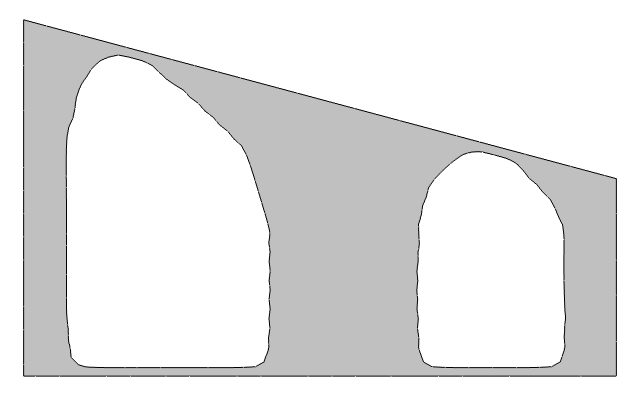
\includegraphics[width=\linewidth]{extriangle.png}
    \end{subfigure}
    \caption{Examples of resulting topologies from COMSOL.}
  \end{figure}

\begin{figure}
  \begin{subfigure}{0.45\textwidth}
    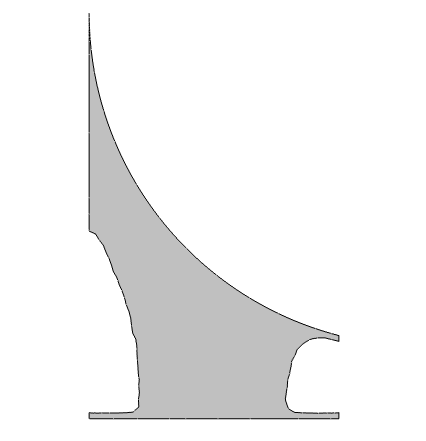
\includegraphics[width=\linewidth]{exround.png}
  \end{subfigure}
  \begin{subfigure}{0.45\textwidth}
      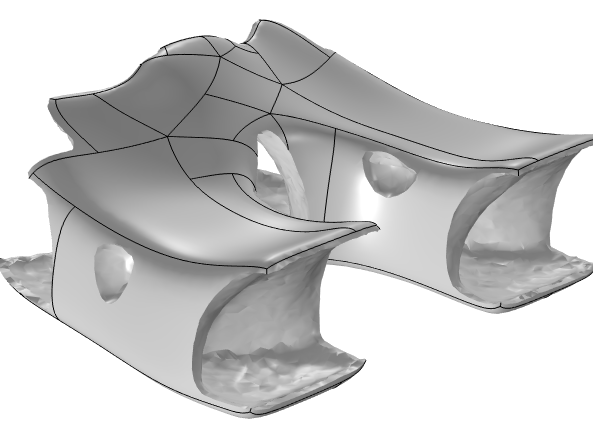
\includegraphics[width=\linewidth]{exfemoral.png}
    \end{subfigure}
  \caption{More examples.}
\end{figure}

\section{Support structure design and merging with part}

After COMSOL was used to generate the possible topologies for the support structure, the topology was exported to image files, in the case of the 2D problem, and to an .STL file, in the case of the 3D structure. These were then converted to 3D .stp file with the aid of FreeCAD. nTop Software was then used to merge the resulting support structure with the manufactured components. Once the support structure and the part were joined, they were exported as .stl files to be used in the SLM finite element simulation.

Once the CAD file of the component and the support structure has been built, it is necessary to merge them together and import them into Simufact to undergo simulation of the manufacturing process. The software used for blending the component and its support structure is nTop version 5.17.2. nTop's interface makes it very easy to merge the part, and also allows to blend the support structure and the component, which effectively creates a fillet between the nodes of both components to allow for a smooth transition between bodies. Of course, blending the component and the support structure in this manner would not give any benefit in a real manufacturing process, as the structure and the component would not be able to be separated easily. Nevertheless, this blend radius is beneficial for the simulation since it was observed that a direct union and import of the support structure + component in Simufact resulted in having very small gaps between the two pieces, resulting in a non manifold geometry that would cause the finite element model to have gaps between some of its nodes.

\begin{figure}
  \begin{subfigure}{0.45\textwidth}
    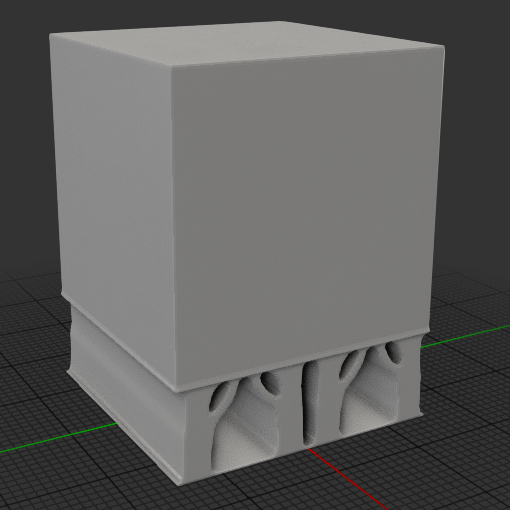
\includegraphics[width=\linewidth]{meldcube.png}
  \end{subfigure}
  \begin{subfigure}{0.45\textwidth}
      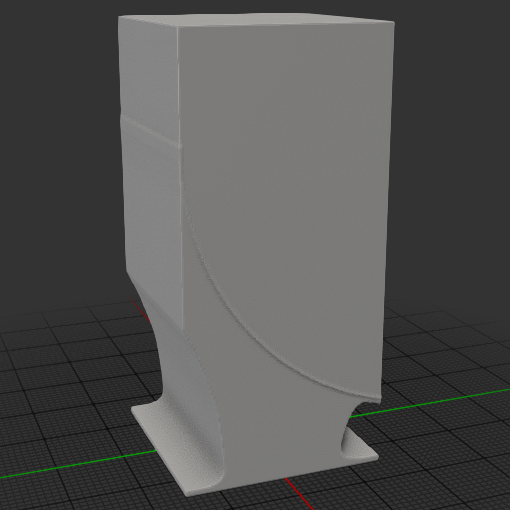
\includegraphics[width=\linewidth]{meldround.png}
    \end{subfigure}
    \caption{Melds of support structures for cube and rounded part.}
  \end{figure}

\begin{figure}
  \begin{subfigure}{0.45\textwidth}
    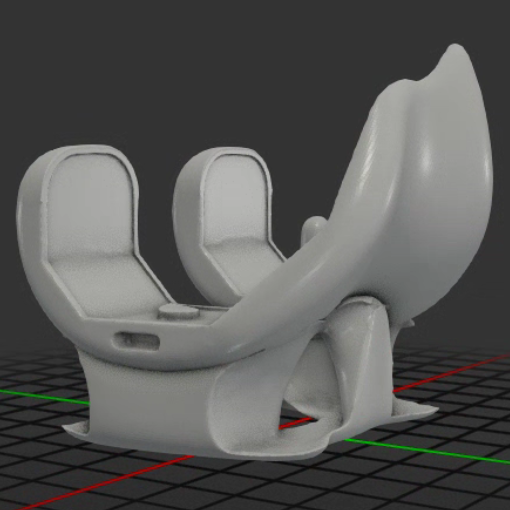
\includegraphics[width=\linewidth]{meldfemoral1.png}
  \end{subfigure}
  \begin{subfigure}{0.45\textwidth}
      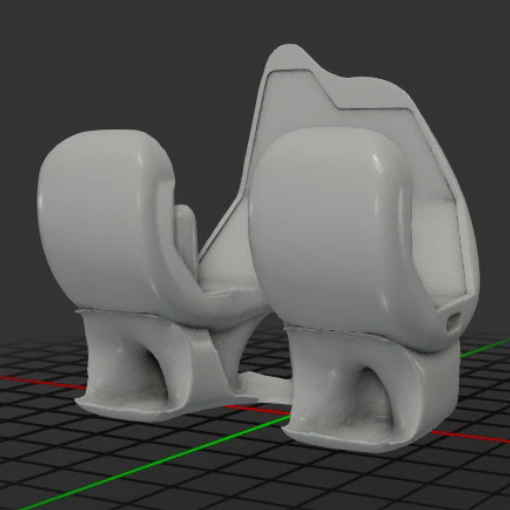
\includegraphics[width=\linewidth]{meldfemoral2.png}
    \end{subfigure}
  \caption{Meld of supporting structure for femoral component.}
\end{figure}

\section{Simulation of manufacturing process}

The software utilized to simulate the manufacturing process is Simufact Additive version 2023.2. Simufact Additive is capable of simulation building process of additive manufacturing components, and coupling thermal and stress physics to predict the temperature values of the component throughout the building process and the total stresses, strains and deformations resulting from the manufacturing process. 

\subsection{Process properties}

After the component and the support structures were merged, they were imported into Simufact. It is during this step that all the factors related to the simulation are set, which include the machine properties, material properties, and build parameters. 

The first parameter to be chosen is the process properties, which determines the physics that Simufact takes into consideration to run the simulation. Simufact provides three different types of processes: mechanical, thermal, and thermomechanical. As stated in the Simufact manual \cite{hexagonabProcessPropertiesInfosheet}, mechanical provides a fast mechanical analysis that only uses inherent strains as the main input. This type of analysis does not take into consideration the temperature fields during the building process. The thermal process on the other hand only considers the thermal behaviour of the components, and the temperature field of the support structures, components and base can be analyzed. The thermomechanical process couples the stress and thermal analyses, and allows for the prediction of temperature, distortions and stresses of the part. This latter thermomechanical process is the process utilized throughout this study.

\subsection{Machine and build parameters}

After choosing the process property, the machine parameters must be specified. This includes the machine build plate geometry and the laser parameters. The machine build plate chosen was a circular plate with an 80 mm radius. The build space dimensions consists of a space of 160 mm in all three x-y-z directions. As for the laser parameters, the simulations were carried out with one laser with a maximum laser power of 500 W and a maximum laser speed of 2000 mm / s, an efficiency of 25\%, and a beam width of 25 mm. These machine parameters were modeled after an AMP-160 SLM machine, manufactured by TongTai Machine \& Tool Company, Taiwan, that has been used in simular studies \cite{chungpei-hsuStudyLatticeSupport2024}, \cite{chungEvaluationPredictionThermal2024a}.

The building parameters for the process need also to be set. These include material layer parameters and any thermal parameters and temperature specifications for the build environment and base plate. The powder layer thickness was chosen to be 0.03 mm, with a recoater time of 10 s. The powder initial temperature was set to 25\degree C, with an initial base temperature of 200\degree C. Preheating is important in SLM since it can influence the quality of the microstructure of the component. It has been suggested that a temperature of 200\degree C exhibits higher cooling rates and smaller grain sizes of the microstructure \cite{chowdhuryEffectsPreheatingThermal2024}.

All of the above parameters plus more are summarized in Tables \ref{tab:laser_params}, \ref{tab:scanner_params}, \ref{tab:thermal_params}, and \ref{tab:adv_thermal_params}.

\begin{table}
  \centering
  \begin{tabular}{ |c|c| }
    \hline
    laser power & 200W \\
    \hline
    laser speed & 1000 mm/s \\
    \hline
    efficiency & 25\% \\
    \hline
    beam width & 100 $\mu$m \\
    \hline
    layer thickness & 30 $\mu$m \\
    \hline
    recoater time & 10 s \\
    \hline
  \end{tabular}
  \caption{Laser parameters}
  \label{tab:laser_params}
\end{table}

\begin{table}
  \centering
  \begin{tabular}{ |c|c| }
    \hline
    scan width & 20 mm \\
    \hline
    scan overlap & 0 mm \\
    \hline
    hatch distance & 0.07 mm \\
    \hline
    pause time & 0 s \\
    \hline
  \end{tabular}
  \caption{Scanner parameters}
  \label{tab:scanner_params}
\end{table}

\begin{table}
  \centering
  \begin{tabular}{ |c|c| }
    \hline
    powder temperature & 25\degree C \\
    \hline
    chamber temperature & 50\degree C \\
    \hline
    base plate temperature & 200\degree C \\
    \hline
  \end{tabular}
  \caption{Thermal parameters}
  \label{tab:thermal_params}
\end{table}

\begin{table}
  \centering
  \begin{tabular}{ |c|c| }
    \hline
    Part / Support emissivity & 0.85 \\
    \hline
    Part / Support heat transfer coefficient & 12.0 W/(m$^2$$\cdot$K) \\
    \hline
    Base plate emissivity & 0.6 \\
    \hline
    Base plate heat transfer coefficient & 20 W/(m$^2$$\cdot$K) \\
    \hline
    Base plate contact heat transfer coefficient & 100 W/(m$^2$$\cdot$K)\\
    \hline
  \end{tabular}
  \caption{Advanced thermal parameters}
  \label{tab:adv_thermal_params}
\end{table}

\subsection{Convergence analysis}

To ensure that FEM results were not dependent on the voxel size of the voxel mesh, a convergence analysis was first performed on one of the simple geometries. For this analysis, the results of three projects were compared. The details of the projects are shown in Table \ref{tab:convergence}. The convergence test proved highly successful, as there is very little difference in the results of the FEM simulations between the different voxel sizes of each project. The results of the convergence test are shown in figure \ref{fig:convergence}. The graphs shows the average and max node deformation of the part's surface, as the voxel size is varied from 1 mm to 0.5 mm. We can see that the variability of surface results due to the voxel size is at most 0.01 mm. In subsequent analyses, the difference between average node displacements of parts with different support structures would be of an order of magnitude bigger ( > 0.1 mm), and thus we can discard the possibility that differences in results are caused or are dependent on the voxel mesh size.

\begin{table}[h!]
  \centering
  \begin{tabular}{|c|c|c|c|c|}
    \hline
    \textbf{Part} & \textbf{Volfrac} & \textbf{tanh($\theta$)} & \textbf{Objective weights} & \textbf{Side density} \\
    \hline
   Cube 1 & 50\% & 0\degree & w1=w2=0.5 & Solid\\
    \hline 
    Cube 2 & 75\% & 4\degree & w1=w2=0.5 & Void\\
    \hline
    Triangle 15\degree & 50\% & 0\degree & w1=w2=0.5 & Solid \\
    \hline
  \end{tabular}
  \caption{Parameters of support structures and geometries for convergence study.}
  \label{tab:convergence}
\end{table}

\begin{figure}
  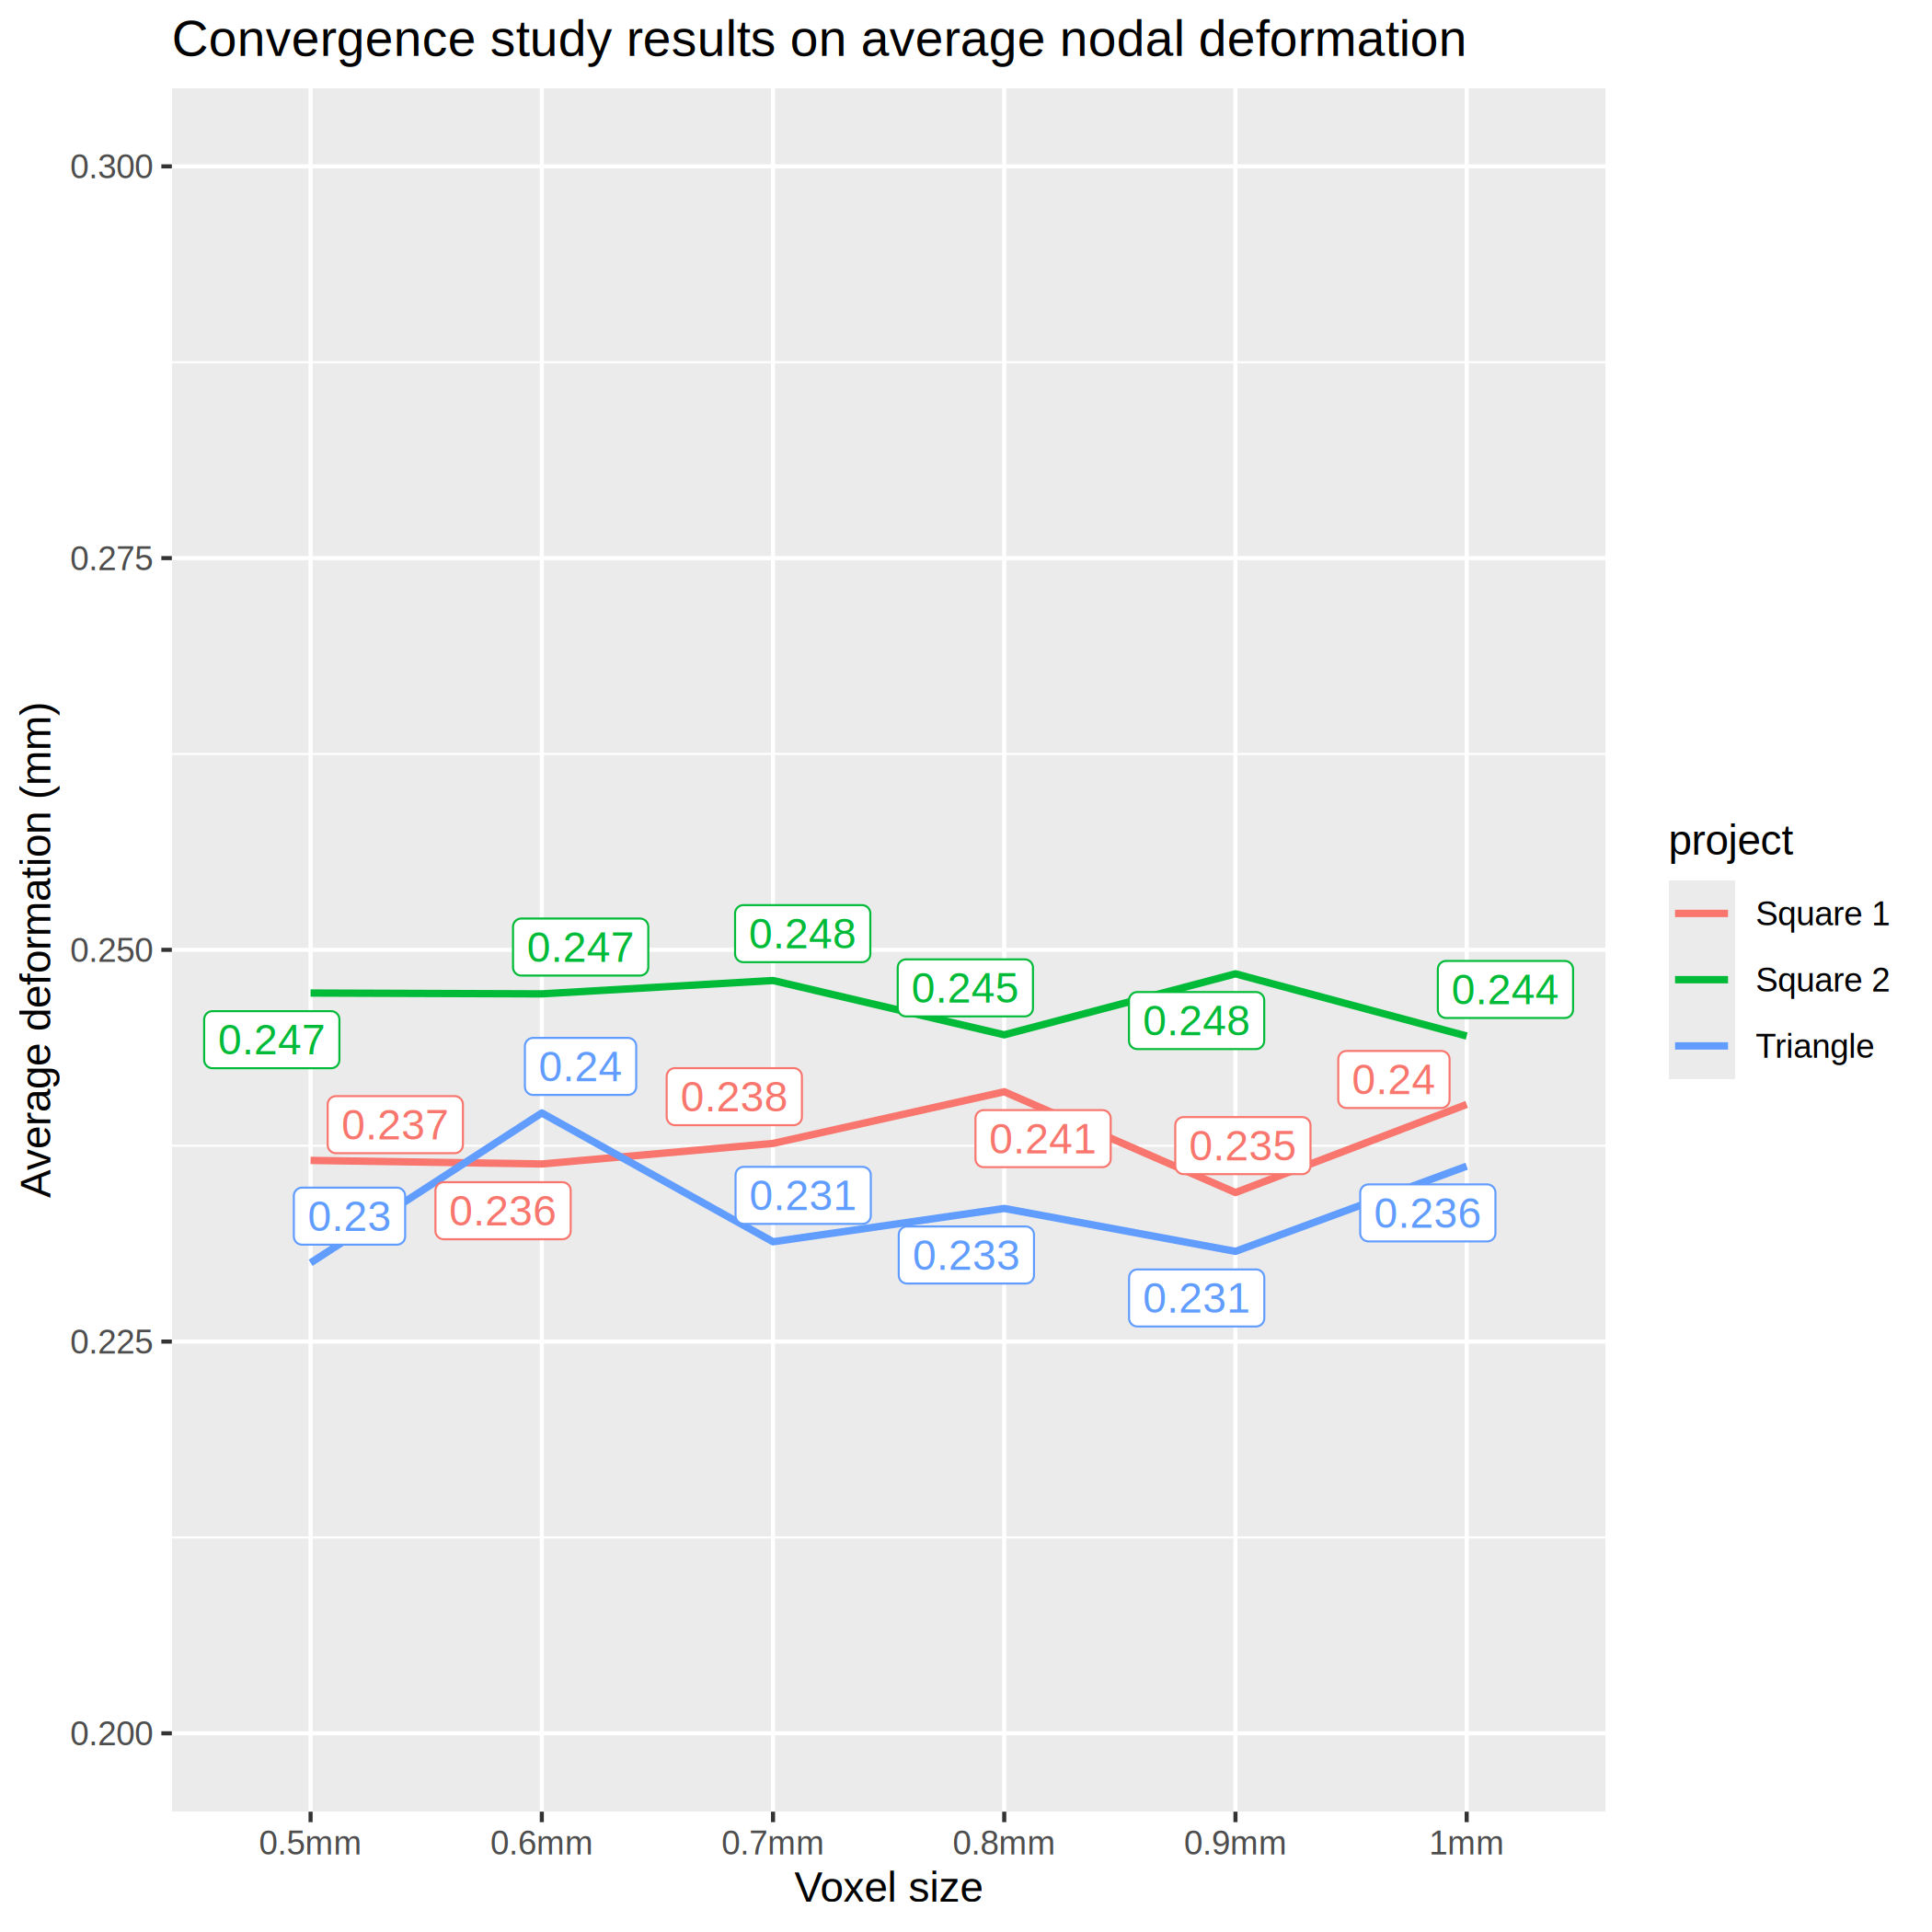
\includegraphics[width=.50\textwidth]{conv_average.png} \hfill
  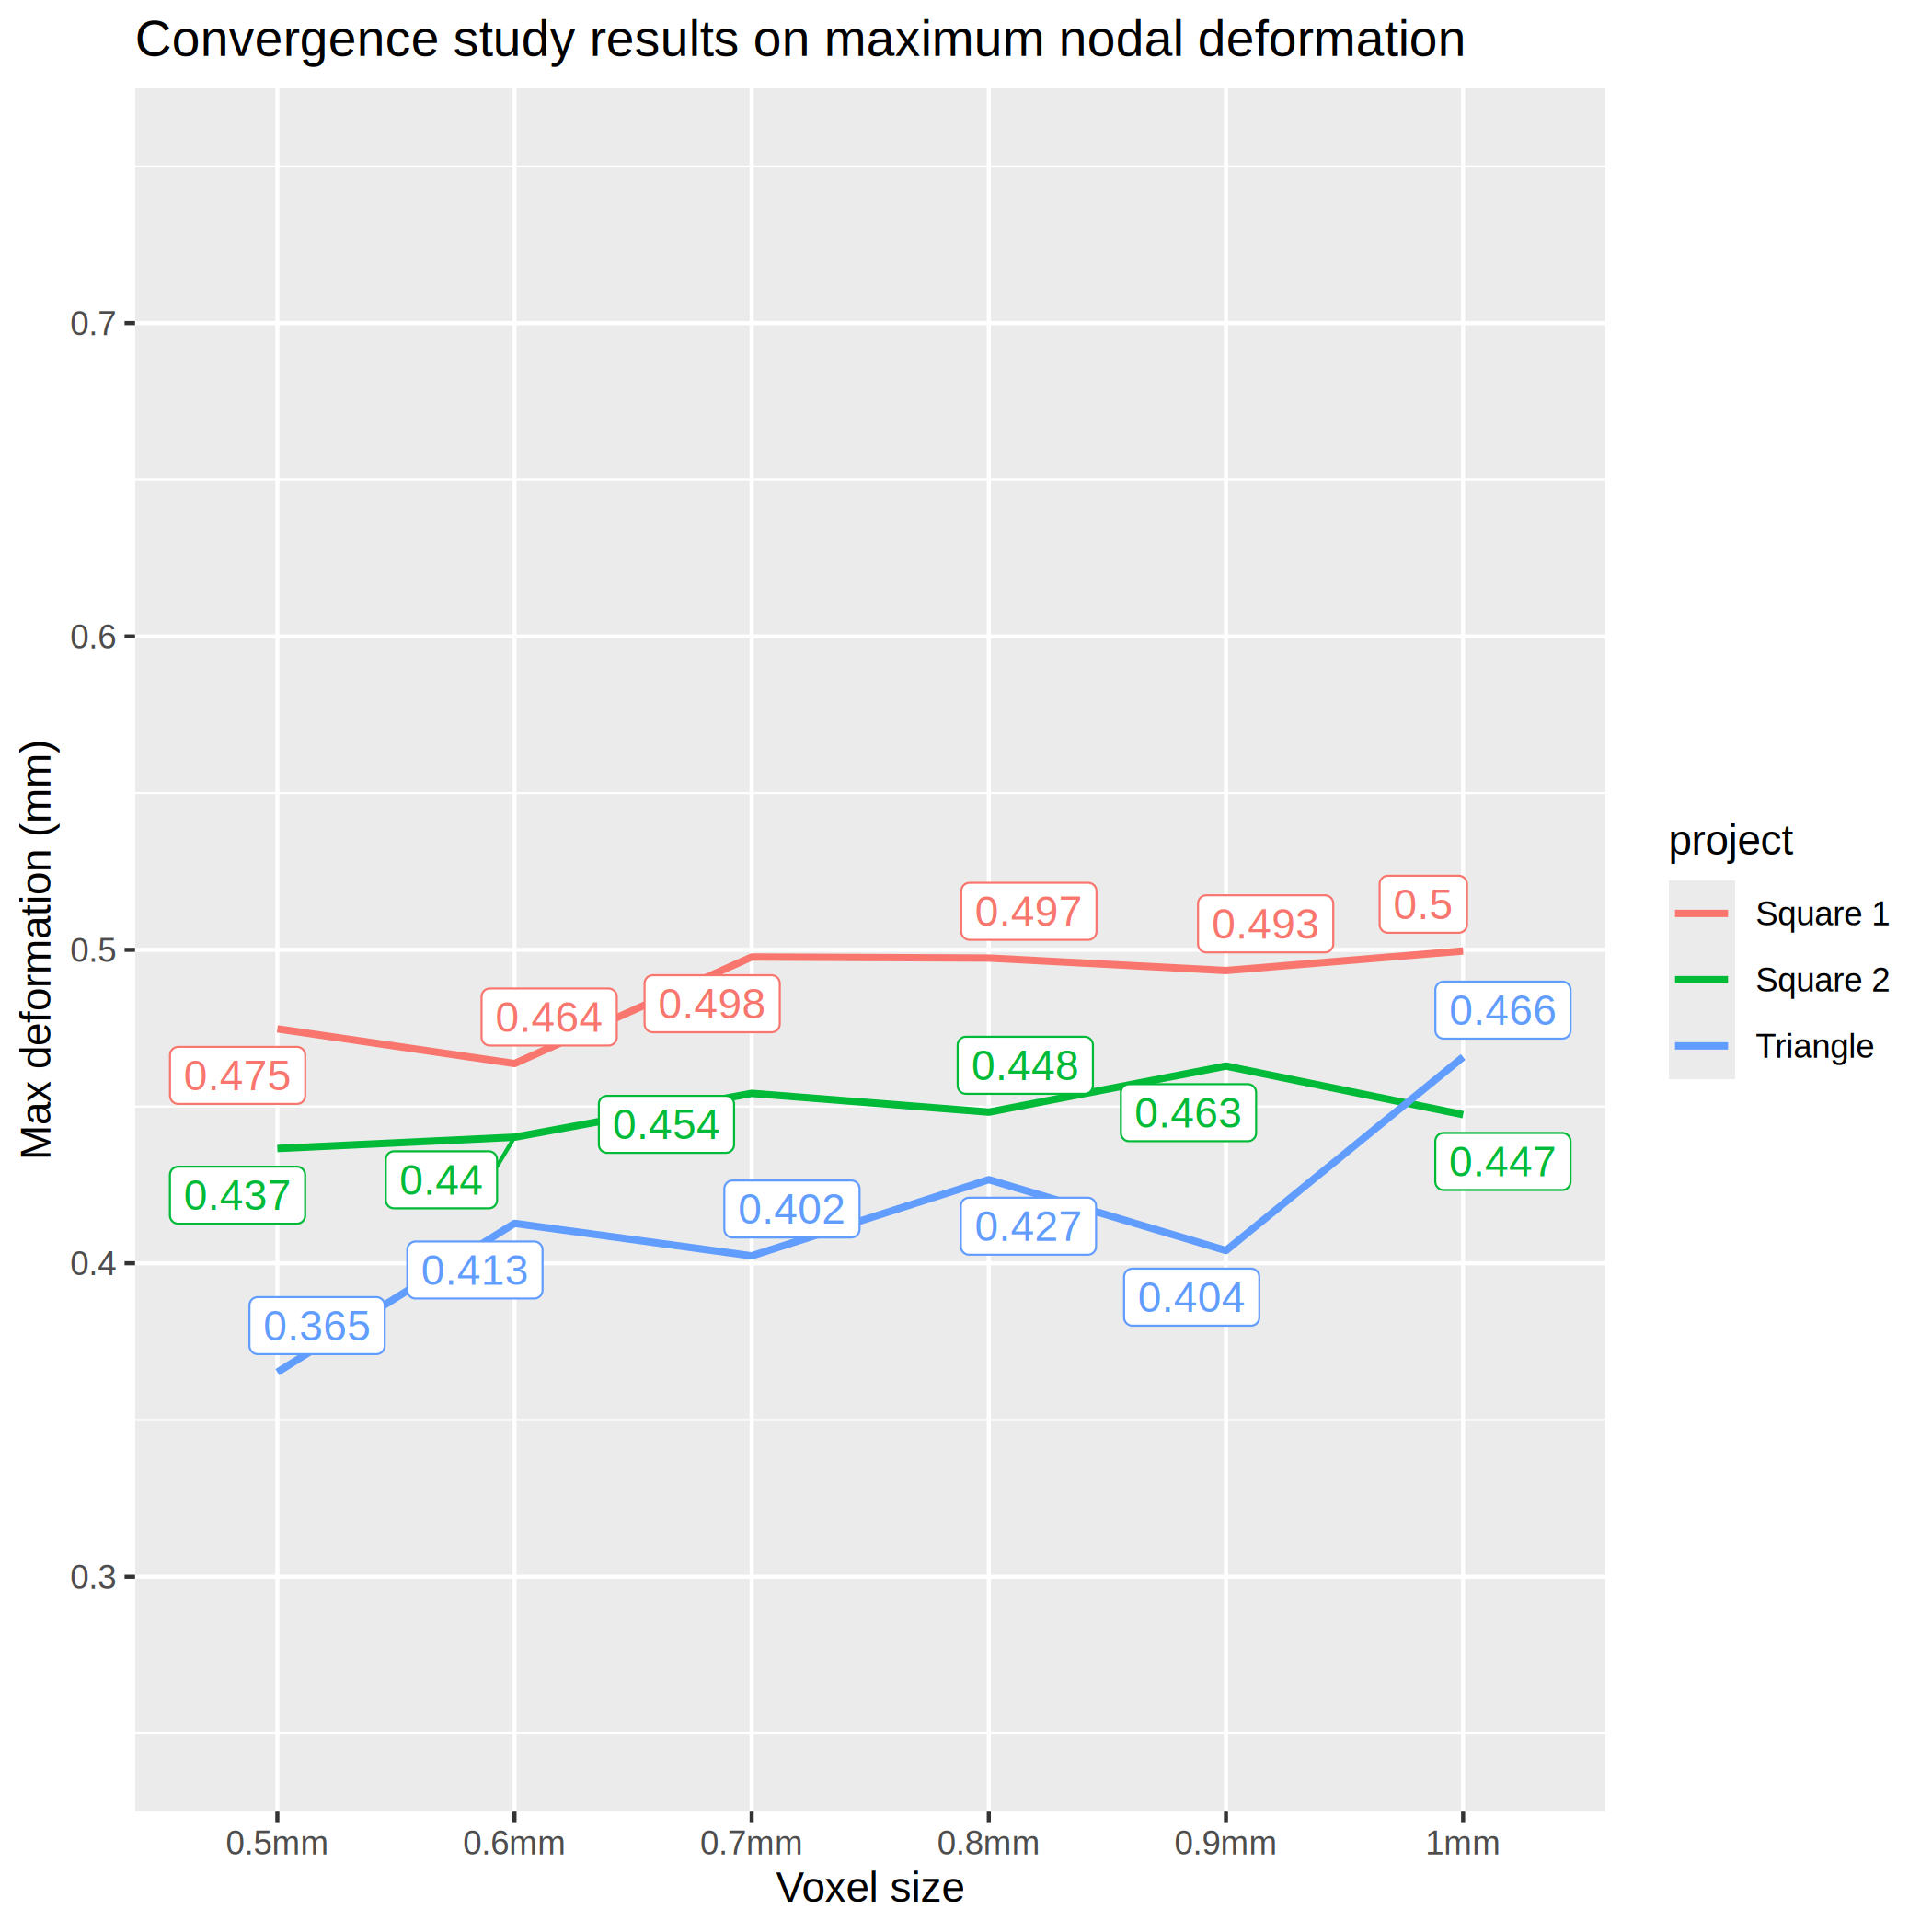
\includegraphics[width=.50\textwidth]{conv_max.png} \hfill
  \caption{Results of convergence test on selected parts.}\label{fig:convergence}
\end{figure} 

\subsection{Voxelization and numerical parameters}

All of the simulations run on Simufact used voxel meshes with sizes ranging from 0.8 mm to 1.5 mm, depending on the complexity of the geometry of the part. The voxelization of the components was performed with Simufact's default voxelization engine. The voxel meshes of the components were uniform in size, while the base plate voxel mesh used adaptive meshing, with 2 levels of coarsening. The solver used for all simulations was the MUMPS Parallel Direct Solver, with 14 time steps for each voxel layer. The voxelization of the femoral component can be seen in Figure \ref{fig:femvox}.

\begin{figure}[h!]
  \centering
  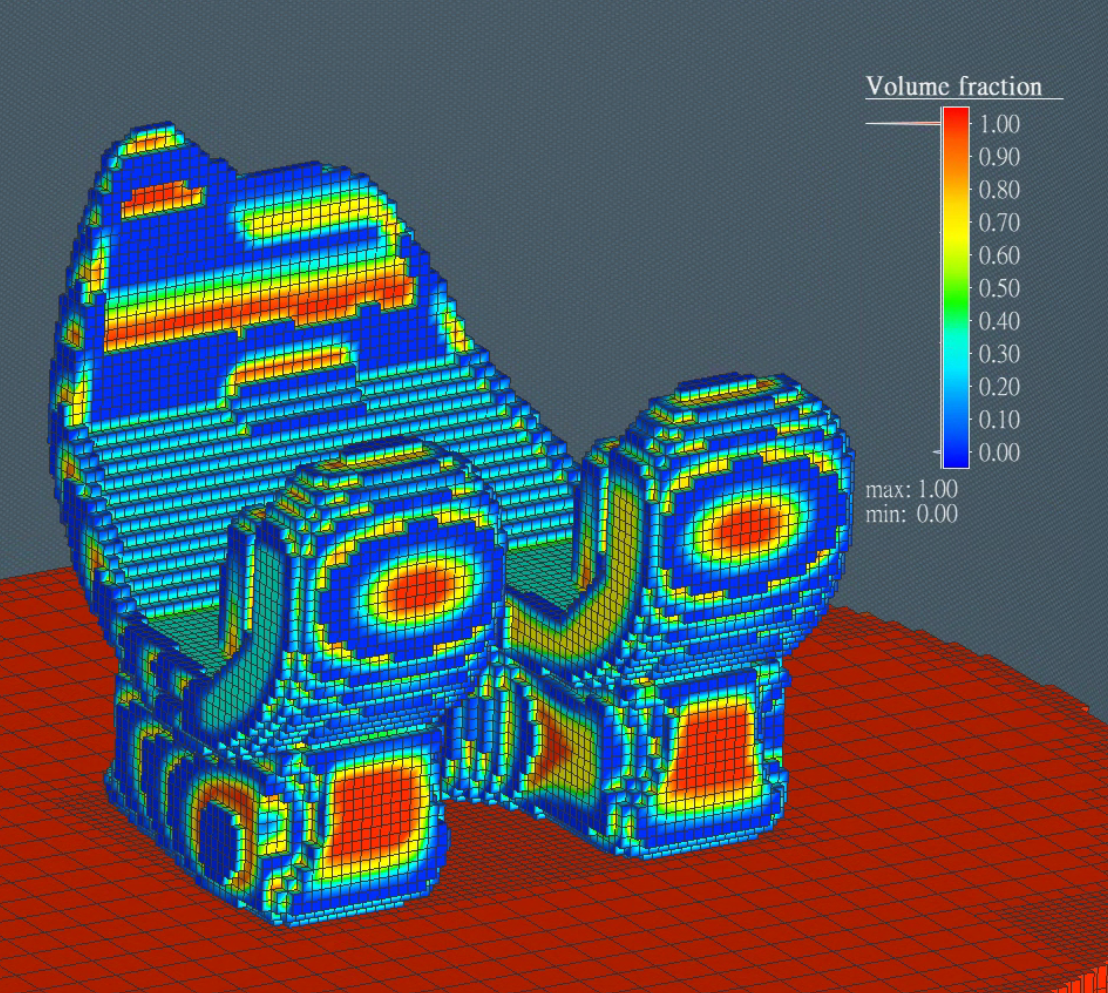
\includegraphics[width=0.8\textwidth]{voxel.png}
  \caption{Voxelization of femoral component in Simufact.}
  \label{fig:femvox}
\end{figure}

\section{Results export and analysis}

After the simulation was run, the node displacement and stress data of last time increment was exported to a .csv file using a Python script. The .csv file was then read and parsed using R, and the data was used to obtain statistical values and graphs. Python code and the R scripts have been included in the Code chapter of this work. \todo{Add this chapter and the code}

\listoftodos

\end{document}
